\documentclass[12pt, leqno]{article} %% use to set typesize
\usepackage{fancyhdr}
\usepackage[letterpaper=true,colorlinks=true,linkcolor=black]{hyperref}

\usepackage{amsfonts}
\usepackage{amsmath,amssymb,amsthm}
\usepackage{color}
\usepackage{tikz}
\usepackage{pgfplots}
\usepackage{listings}
%\usepackage{courier}
%\usepackage[utf8]{inputenc}
%\usepackage[russian]{babel}

\lstdefinelanguage{Julia}%
  {morekeywords={abstract,break,case,catch,const,continue,do,else,elseif,%
      end,export,false,for,function,immutable,import,importall,if,in,%
      macro,module,otherwise,quote,return,switch,true,try,type,typealias,%
      using,while},%
   sensitive=true,%
   alsoother={$},%
   morecomment=[l]\#,%
   morecomment=[n]{\#=}{=\#},%
   morestring=[s]{"}{"},%
   morestring=[m]{'}{'},%
}[keywords,comments,strings]%

\lstset{
  numbers=left,
  basicstyle=\ttfamily\footnotesize,
  numberstyle=\tiny\color{gray},
  stepnumber=1,
  numbersep=10pt,
}

\newcommand{\iu}{\ensuremath{\mathrm{i}}}
\newcommand{\bbR}{\mathbb{R}}
\newcommand{\bbC}{\mathbb{C}}
\newcommand{\calV}{\mathcal{V}}
\newcommand{\calE}{\mathcal{E}}
\newcommand{\calG}{\mathcal{G}}
\newcommand{\calW}{\mathcal{W}}
\newcommand{\calP}{\mathcal{P}}
\newcommand{\macheps}{\epsilon_{\mathrm{mach}}}
\newcommand{\matlab}{\textsc{Matlab}}
\newcommand{\uQ}{\underline{Q}}
\newcommand{\uR}{\underline{R}}

\newcommand{\ddiag}{\operatorname{diag}}
\newcommand{\fl}{\operatorname{fl}}
\newcommand{\nnz}{\operatorname{nnz}}
\newcommand{\tr}{\operatorname{tr}}
\renewcommand{\vec}{\operatorname{vec}}

\newcommand{\vertiii}[1]{{\left\vert\kern-0.25ex\left\vert\kern-0.25ex\left\vert #1
    \right\vert\kern-0.25ex\right\vert\kern-0.25ex\right\vert}}
\newcommand{\ip}[2]{\langle #1, #2 \rangle}
\newcommand{\ipx}[2]{\left\langle #1, #2 \right\rangle}
\newcommand{\order}[1]{O( #1 )}

\newcommand{\kron}{\otimes}


\newcommand{\hdr}[1]{
  \pagestyle{fancy}
  \lhead{Bindel, Fall 2022}
  \rhead{Matrix Computations}
  \fancyfoot{}
  \begin{center}
    {\large{\bf #1}}
  \end{center}
  \lstset{language=Julia,columns=flexible}  
}


\begin{document}

\hdr{2022-09-22}

\section{A family of factorizations}

\subsection{Cholesky}

If $A \in \mathbb{R}^{m \times n}$ with $m > n$ is full rank, then
$A^T A$ is symmetric and positive definite matrix, and we can compute
a Cholesky factorization of $A^T A$:
\[
  A^T A = R^T R.
\]
The solution to the least squares problem is then
\[
  x = (A^T A)^{-1} A^T b = R^{-1} R^{-T} A^T b.
\]
Or, in Julia world
\begin{lstlisting}
  F = chol(A'*A);
  x = F\(A'*b);
\end{lstlisting}

\subsection{Economy QR}

The Cholesky factor $R$ appears in a different setting as well.
Let us write $A = QR$ where $Q = AR^{-1}$; then
\[
  Q^T Q = R^{-T} A^T A R^{-1} = R^{-T} R^T R R^{-1} = I.
\]
That is, $Q$ is a matrix with orthonormal columns.  This
``economy QR factorization'' can be computed in several different
ways, including one that you have seen before in a different guise
(the Gram-Schmidt process).

Julia provides a numerically stable
method to compute the QR factorization via
\begin{lstlisting}
  F = qr(A)
\end{lstlisting}
and we can use the QR factorization directly to solve the least
squares problem without forming $A^T A$ by
\begin{lstlisting}
  F = qr(A)
  x = F\b
\end{lstlisting}
Behind the scenes, this is what is used when we write \verb|A\b| with
a dense rectangular matrix $A$.

\subsection{Full QR}

There is an alternate ``full'' QR decomposition where we write
\[
A = QR, \mbox{ where }
Q = \begin{bmatrix} Q_1 & Q_2 \end{bmatrix} \in \bbR^{n \times n},
R = \begin{bmatrix} R_{1} \\ 0 \end{bmatrix} \in \bbR^{m \times n}.
\]
To see how this connects to the least squares problem, recall
that the Euclidean norm is invariant under orthogonal transformations,
so
\[
  \|r\|^2 = \|Q^T r\|^2 = \left\| \begin{bmatrix} Q_1^T b \\ Q_2^T
    b \end{bmatrix} - \begin{bmatrix} R_1 \\ 0 \end{bmatrix} x
  \right\|^2 = \|Q_1^T b-R_1x\|^2 + \|Q_2^T b\|^2.
\]
We can set $\|Q_1^T v-R_1 x\|^2$ to zero by
setting $x = R_1^{-1} Q_1^T b$; the result is
$\|r\|^2 = \|Q_2^T b\|^2$.

The QR factorization routine in Julia can be used to reconstruct
either the full or the compact QR decomposition.  Internally, it
stores neither the smaller $Q_1$ nor the full matrix $Q$ explicitly;
rather, it uses a compact representation of the matrix as a product of
Householder reflectors, as we will discuss next time.

\subsection{SVD}

The full QR decomposition is useful because orthogonal transformations
do not change lengths.  Hence, the QR factorization lets us change
to a coordinate system where the problem is simple without changing
the problem in any fundamental way.  The same is true of the SVD,
which we write as
\begin{align*}
A &=
\begin{bmatrix} U_1 & U_2 \end{bmatrix}
\begin{bmatrix} \Sigma \\ 0 \end{bmatrix}
V^T & & \mbox{Full SVD} \\
&= U_1 \Sigma V^T & & \mbox{Economy SVD}.
\end{align*}
As with the QR factorization, we can apply an orthogonal
transformation involving the factor $U$ that makes the
least squares residual norm simple:
\[
\|U^T r\|^2 =
\left\| \begin{bmatrix} U_1^T b \\ U_2^T b \end{bmatrix} -
\begin{bmatrix} \Sigma V^T \\ 0 \end{bmatrix} x
\right\| =
\|U_1^T b - \Sigma V^T x\|^2 + \|U_2^T b\|^2,
\]
and we can minimize by setting $x = V \Sigma^{-1} U_1^T b$.

\section{QR and Gram-Schmidt}

We now turn to our first numerical method for computing the
QR decomposition: the Gram-Schmidt algorithm.  This method is
usually presented in first linear algebra classes, but is
rarely interpreted as a matrix factorization.  Rather, it is
presented as a way of converting a basis for a space into an
orthonormal basis for the same space.  If $a_1, a_2, \ldots, a_n$
are column vectors, the Gram-Schmidt algorithm is as follows:
for each $j = 1, \ldots, n$
\begin{align*}
  \tilde{a}_j &= a_j - \sum_{i=1}^{j-1} q_i q_i^T a_j \\
  q_j &= \tilde{a}_j / \|\tilde{a}\|_j.
\end{align*}
At the end of the iteration, we have that the $q_j$ vectors are
all mutually orthonormal and
\[
  \operatorname{span}\{ a_1, \ldots, a_j \} =
  \operatorname{span}\{ q_1, \ldots, q_j \}.
\]
To see this as a matrix factorization, we rewrite the iteration as
\begin{align*}
  r_{ij} &= q_i^T a_j \\
  \tilde{a}_j &= a_j - \sum_{i=1}^{j-1} q_i r_{ij} \\
  r_{jj} &= \|\tilde{a}\|_j \\
  q_j &= \tilde{a}_j / r_{jj}
\end{align*}
Putting these equations together, we have that
\[
  a_j = \sum_{i=1}^j q_i r_{ij},
\]
or, in matrix form,
\[
  A = QR
\]
where $A$ and $Q$ are the matrices with column vectors $a_j$ and $q_j$,
respectively.

In Julia, Gram-Schmidt looks
something like this:
\begin{lstlisting}
function orth_cgs0(A)
    m,n = size(A)
    Q = zeros(m,n)
    for j = 1:n
        v = A[:,j]                        # Take the jth original basis vector
        v = v-Q[:,1:j-1]*(Q[:,1:j-1]'*v)  # Orthogonalize vs q_1, ... q_j-1
        v = v/norm(v)                     # Normalize what remains
        Q[:,j] = v                        # Add result to Q basis
    end
    Q
end
\end{lstlisting}

Where does $R$ appear in this algorithm?  It appears thus:
\begin{lstlisting}
function orth_cgs(A)
    m,n = size(A)
    Q = zeros(m,n)
    R = zeros(n,n)
    for j = 1:n
        v = A[:,j]                        # Take the jth original basis vector
        R[1:j-1,j] = Q[:,1:j-1]'*v        # Project onto q_1, ..., q_j-1
        v = v-Q[:,1:j-1]*R[1:j-1,j]       # Orthogonalize vs q_1, ... q_j-1
        R[j,j] = norm(v)                  # Compute normalization constant
        v = v/R[j,j]                      # Normalize what remains
        Q[:,j] = v                        # Add result to Q basis
    end
    Q, R
end
\end{lstlisting}
That is, $R$ accumulates the multipliers that we computed from
the Gram-Schmidt procedure.  This idea that the multipliers
in an algorithm can be thought of as entries in a matrix should
be familiar, since we encountered it before when we looked at
Gaussian elimination.

Sadly, the Gram-Schmidt algorithm is not backward stable.
The problem occurs when a vector $a_j$ is nearly in the span of
previous vectors, so that cancellation rears its ugly head in the
formation of $\tilde{a}_j$.  As a result, we have that $A+E = \hat{Q} \hat{R}$ is
usually satisfied with a relatively small $E$, but
$\|\hat{Q}^T \hat{Q}-I\|$ may not be small (in the worst case, the computed
$\hat{Q}$ may even be near singular).
The classical Gram-Schmidt (CGS) method that we have shown is particularly
problematic; a somewhat better alternative is the modified Gram-Schmidt
method (MGS) algorithm:
\begin{lstlisting}
function orth_mgs(A)
    m,n = size(A)
    Q = zeros(m,n)
    R = zeros(n,n)
    for j = 1:n
        v = A[:,j]                        # Take the jth original basis vector
        for k = 1:j-1
            R[k,j] = Q[:,j]'*v            # Project onto q_1, ..., q_j-1
            v -= Q[:,j]*R[k,j]            # Orthogonalize vs q_1, ... q_j-1
        end
        R[j,j] = norm(v)                  # Compute normalization constant
        v = v/R[j,j]                      # Normalize what remains
        Q[:,j] = v                        # Add result to Q basis
    end
    Q, R
end
\end{lstlisting}
Though equivalent in exact arithmetic, the MGS algorithm has the advantage
that it computes dot products with the updated $\tilde{a}_j$ as we go
along, and these intermediate vectors have smaller norm than the original
vector.  Sadly, this does not completely fix the matter: the computed $q_j$
vectors can still drift away from being orthogonal to each other.  One can
explicitly re-orthogonalize vectors that drift away from orthogonality,
and this helps further.  In practice, though, we usually don't bother: if
backward stability is required, we turn to other algorithms.

Despite its backward instability, the Gram-Schmidt algorithm forms a very
useful building block for iterative methods, and we will see it frequently
in later parts of the course.

\section{Householder transformations}

The Gram-Schmidt orthogonalization procedure is not generally
recommended for numerical use.  Suppose we write $A = [a_1 \ldots
  a_m]$ and $Q = [q_1 \ldots q_m]$.  The essential problem is that if
$r_{jj} \ll \|a_j\|_2$, then cancellation can destroy the accuracy of
the computed $q_j$; and in particular, the computed $q_j$ may not be
particularly orthogonal to the previous $q_j$.  Actually, loss of
orthogonality can build up even if the diagonal elements of $R$ are
not exceptionally small.  This is Not Good, and while we have some
tricks to mitigate the problem, we need a different approach if we
want the problem to go away.

Recall that one way of expressing the Gaussian elimination algorithm
is in terms of Gauss transformations that serve to introduce zeros
into the lower triangle of a matrix.  {\em Householder} transformations
are orthogonal transformations (reflections) that can be used to similar
effect.  Reflection across the plane orthogonal to a unit normal
vector $v$ can be expressed in matrix form as
\[
  H = I-2 vv^T.
\]

Now suppose we are given a vector $x$ and we want to find a reflection
that transforms $x$ into a direction parallel to some unit vector $y$.
The right reflection is through a hyperplane that bisects the angle
between $x$ and $y$ (see Figure~\ref{fig1}), which we can construct
by taking the hyperplane normal to $x-\|x\|y$.  That is,
letting $u = x - \|x\|y$ and $v = u/\|u\|$, we have
\begin{align*}
  (I-2vv^T)x
  & = x - 2\frac{(x+\|x\|y)(x^T x + \|x\| x^T y)}{\|x\|^2 + 2 x^T y \|x\| + \|x\|^2 \|y\|^2} \\
  & = x - (x-\|x\|y) \\
  & = \|x\|y.
\end{align*}
If we use $y = \pm e_1$, we can get a reflection that zeros out all but the
first element of the vector $x$.  So with appropriate choices of reflections,
we can take a matrix $A$ and zero out all of the subdiagonal elements
of the first column.

\begin{figure}
\begin{center}
  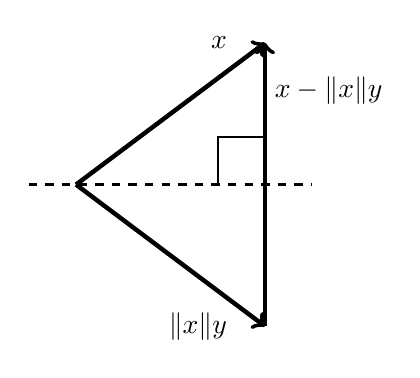
\begin{tikzpicture}[scale=0.6]
    \draw [thick,dashed] (-1,0) -- (5,0);
    \draw [ultra thick,->] (0,0) -- (4,3);
    \draw [ultra thick,->] (0,0) -- (4,-3);
    \draw [ultra thick,->] (4,-3) -- (4,3);
    \draw [thick] (3,0) -- (3,1) -- (4,1);
    \draw (4,2) node [right] {$x-\|x\| y$};
    \draw (3.4,3) node [left] {$x$};
    \draw (3.4,-3) node [left] {$\|x\| y$};
  \end{tikzpicture}
\end{center}
\caption{Construction of a reflector to transform $x$ into $\|x\|y$,
         $\|y\| = 1$.}
\label{fig1}
\end{figure}

Now think about applying a sequence of Householder transformations to
introduce subdiagonal zeros into $A$, just as we used a sequence of Gauss
transformations to introduce subdiagonal zeros in Gaussian elimination.
As with $LU$ factorization, we can re-use the storage of $A$ by recognizing
that the number of nontrivial parameters in the vector $w$ at each step
is the same as the number of zeros produced by that transformation.
This gives us the following:
\begin{lstlisting}
function hqr!(A)
    m,n = size(A)
    tau = zeros(n)

    for j = 1:n

        # Find H = I-tau*w*w' to zero out A[j+1:end,j]
        normx = norm(A[j:end,j])
        s     = -sign(A[j,j])
        u1    = A[j,j] - s*normx
        w     = A[j:end,j]/u1
        w[1]  = 1.0
        A[j+1:end,j] = w[2:end]   # Save trailing part of w
        A[j,j] = s*normx          # Diagonal element of R
        tau[j] = -s*u1/normx      # Save scaling factor

        # Update trailing submatrix by multipling by H
        A[j:end,j+1:end] -= tau[j]*w*(w'*A[j:end,j+1:end])

    end

    A, tau
end
\end{lstlisting}

If we ever need $Q$ or $Q^T$ explicitly, we can always form it from
the compressed representation.  We can also multiply by $Q$ and $Q^T$
implicitly:
\begin{lstlisting}
function applyQ!(QR, τ, X)
    m, n = size(QR)
    for j = n:-1:1
        w = [1.0; QR[j+1:end,j]]
        X[j:end,:] -= tau[j]*w*(w'*X[j:end,:])
    end
    X
end

function applyQT!(QR, τ, X)
    m, n = size(QR)
    for j = 1:n
        w = [1.0; QR[j+1:end,j]]
        X[j:end,:] -= tau[j]*w*(w'*X[j:end,:])
    end
    X
end

applyQ(QR, tau, X) = applyQ!(QR, tau, copy(X))
applyQT(QR, tau, X) = applyQ(QR, tau, copy(X))
\end{lstlisting}


\section{Block reflectors}

As with Gaussian elimination, we would prefer to have a block
implementation of the algorithm available in order to get better use
of level 3 BLAS routines.  To do this, we seek a representation for a
block reflector.  Three such representations are common in the
literature:
\begin{itemize}
\item The block reflector (or $GG^T$) representation: $H = I-2UU^T$
\item The $WY^T$ representation: $H = I + WY^T$ where $W$ and $Y$ are
  computed via a recurrence relation
\item The compact $WY^T$ representation: $H = I + YTY^T$ where $T$ is
  upper triangular
\end{itemize}
The LAPACK routine {\tt DGEQRT} uses the compact $WY^T$ representation, as
do most variants of the {\tt qr} routine in Julia.

\section{Givens rotations}

Householder reflections are one of the standard orthogonal
transformations used in numerical linear algebra.  The other standard
orthogonal transformation is a {\em Givens rotation}:
\[
  G = \begin{bmatrix}
    c & -s \\
    s & c
  \end{bmatrix}.
\]
where $c^2 + s^2 = 1$.  Note that
\[
  G = \begin{bmatrix}
    c & -s \\
    s & c
  \end{bmatrix}
  \begin{bmatrix}
    x \\ y
  \end{bmatrix} =
  \begin{bmatrix}
    cx - sy \\
    sx + cy
  \end{bmatrix}
\]
so if we choose
\begin{align*}
  s &= \frac{-y}{\sqrt{x^2 + y^2}}, &
  c &= \frac{x}{\sqrt{x^2+y^2}}
\end{align*}
then the Givens rotation introduces a zero in the second column.
More generally, we can transform a vector in $\bbR^m$ into a vector
parallel to $e_1$ by a sequence of $m-1$ Givens rotations, where
the first rotation moves the last element to zero, the second rotation
moves the second-to-last element to zero, and so forth.

For some applications, introducing zeros one by one is very
attractive.  In some places, you may see this phrased as a contrast
between algorithms based on Householder reflections and those based on
Givens rotations, but this is not quite right.  Small Householder
reflections can be used to introduce one zero at a time, too.
Still, in the general usage, Givens rotations seem to be the more
popular choice for this sort of local introduction of zeros.

\section{Stability of QR}

It is not too difficult to show that applying a Givens rotations or
Householder reflector to a matrix is backward-stable: if $P$ is the
desired transformation, the floating point result of $PA$ is
\[
  \tilde{P} A = (P+E) A, \quad \|E\| \leq O(\macheps) \|A\|.
\]
Moreover, orthogonal matrices are perfectly conditioned!
Taking a product of $j$ matrices is also fine; the result
has backward error bounded by $j O(\macheps) \|A\|$.
As a consequence, QR decomposition by Givens rotations or Householder
transformations is ultimately backward stable.

The stability of orthogonal matrices in general makes them a
marvelous building block for numerical linear algebra algorithms,
and we will take advantage of this again when we discuss
eigenvalue solvers.

\section{Sparse QR}

Just as was the case with LU, the QR decomposition admits a sparse
variant.  And, as with LU, sparsity of the
matrix $A \in \bbR^{m \times n}$ alone is not
enough to guarantee sparsity of the factorization!  Hence, as with
solving linear systems, our recommendation for solving sparse least
squares problems varies depending on the actual sparse structure.

Recall that the $R$ matrix in QR factorization is also the Cholesky
factor of the Gram matrix: $G = A^T A = R^T R$.  Hence, the sparsity of
the $R$ factor can be inferred from the sparsity of $G$ using the ideas
we talked about when discussing sparse Cholesky.  If the rows of $A$
correspond to experiments and columns correspond to factors, the nonzero
structure of $G$ is determined by which experiments share common
factors: in general $g_{ij} \neq 0$ if any experiment involves both
factors $i$ and factor $j$. So a very sparse $A$ matrix may nonetheless
yield a completely dense $G$ matrix. Of course, if $R$ is dense, that is
not the end of the world!  Factoring a dense $n \times n$ matrix is
pretty cheap for $n$ in the hundreds or even up to a couple thousand,
and solves with the resulting triangular factors are quite inexpensive.

If one forms $Q$ at all, it is often better to work with $Q$ as a
product of (sparse) Householder reflectors rather than forming the
elements of $Q$.  One may also choose to use a ``$Q$-less QR decomposition''
in which the matrix $Q$ is not kept in any explicit form; to form $Q^T b$
in this case, we would use the formulation $Q^T b = R^{-T} A^T b$.

As with linear solves, least squares solves can be ``cleaned up''
using iterative refinement.  This is a good idea in particular when
using $Q$-less QR.  If $\tilde{A}^\dagger$ is an approximate least
squares solve (e.g.~via the slightly-unstable normal equations approach),
iterative refinement looks like
\begin{align*}
  r^{k} &= b-Ax^{k} \\
  x^{k+1} &= x^k - \tilde{R}^{-1} (\tilde{R}^{-T} (A^T r_k)).
\end{align*}
This approach can be useful even when $A$ is moderately large and dense;
for example, $\tilde{R}$ might be computed from a (scaled) QR
decomposition of a carefully selected subset of the rows of $A$.

\end{document}
